\chapter{Introduction} \label{chapitre-1}

\section{Définition du Neurofeedback}
% voir lambez B et al. 2019

\subsection{Historique}

Le \gls{nfb} est une technique de thérapie comportementale ayant pour but d'apprendre ou d'améliorer l'auto-régulation de l'activité cérébrale.
Les prémices du \gls{nfb} remontent au début des années 1930, peu après l'enregistrement du premier \gls{eeg} humain par Hans Berger en 1929.
En effet, \citet{Durup1935} et \citet{Loomis1936} ont observé que les ondes alpha, oscillant entre 8 et 12Hz, pouvaient être contrôlées grâce au 
conditionnment classique. 

Plus tard, ce qui peut être considéré comme le premier entrainement par \gls{nfb} a été mené par le Dr. Kamiya qui a demandé aux sujets de son étude 
de contrôler le rythme alpha et qui a obtenu des résultats prometteurs \citep{Kamiya1969}. 

Une preuve solide de la modulation de l'\gls{eeg} a été rapportée dans les années 1960 par le Dr. Sterman : l'expérience 
originelle consistait à entrainer le cerveau des chats en leur apprenant quoi faire pour obtenir de 
la nourriture. Durant cette expérience, le Dr. Sterman a extrait un rythme particulier au niveau du cortex sensorimoteur : le \gls{smr}, qui correspond 
aux fréquences entre 12 et 15Hz. Ensuite, le but du Dr. Sterman a été d'entrainer les chats à produire ce rythme en leur donnant de la nourriture 
lorsqu'ils réussissaient à l'émettre pendant une demi seconde, ce que les chats ont vite appris à faire. 

Cette modulation a ensuite été employée à des fins cliniques : l'entrainement du \gls{smr} chez les chats améliore leur sommeil \citep{Sterman1970} mais aussi
réduit la fréquence de leurs crises d'épilepsie après une exposition au kérosène \citep{Sterman1974}. Cependant, le \gls{nfb} ne correspondant pas à ce qui 
était connu à l'époque quant au fonctionnement du cerveau humain, son utilisation s'est faite en marge de la communauté scientifique \citep{Masterpasqua2003}. 
Il faut attendre les années 2000 pour que le \gls{nfb} soit réhabilité conduisant à une explosion du nombre d'études scientifiques visant à mieux comprendre 
ses mécanismes et ses effets, illustrée à la Figure~\ref{Figure:introduction_number_of_nfb_publications}. 

\begin{figure}[h!]
  \centering
	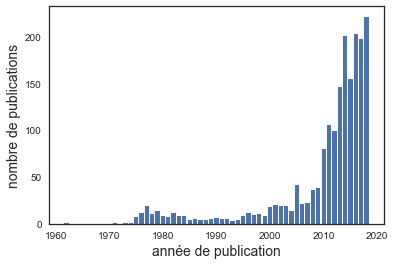
\includegraphics[width=0.7\linewidth]{figures/chapter-1/introduction-number-of-nfb-publications} 
  \caption{Evolution du nombre de publications sur le Neurofeedback par année, entre 1962 et 2018. La base de données PubMed a été questionnée avec les 
	termes de recherche "Neurofeedback OR EEG Biofeedback".}
  \label{Figure:introduction_number_of_nfb_publications}
\end{figure}

\subsection{Principe du Neurofeedback}

Le \gls{nfb} a pour but d'apprendre à un sujet à auto-réguler son activité cérébrale à l'aide de retours auditifs et/ou visuels en temps réel. 
Ces retours lui permettent de suivre la régulation de son rythme cérébral : si elle est modulée de la manière souhaitée, une récompense 
auditive et/ou visuelle est attribuée, sinon le sujet doit prendre une action corrective. Le \gls{nfb} est basé sur le conditionnement opérant 
\citep{Reynolds1975} : celui-ci se distingue du conditionnement classique où un stimulus conduit à une réaction automatique. 
En effet, dans le cas du conditionnement opérant, le conditionnement n'est pas lié à des réponses réflexes de
l'organisme mais à l'influence de l'environnement, qui renforce positivement ou négativement le conditionnement \citep{Skinner1948}. 

L'activité cérébrale enregistrée lors du \gls{nfb} est couramment l'\gls{eeg}, cependant d'autres modalités telles que l'imagerie par résonance 
magnétique fonctionnelle (\gls{fmri} en anglais) \citep{Sulzer2013} ou le couplage entre l'\gls{eeg} et la \gls{fmri} \citep{Perronnet2017} existent. Ici,
on s'intéresse seulement au \gls{nfb} \gls{eeg}. L'\gls{eeg} est enregistré de façon non-invasive au moyen d'électrodes placées sur le scalp, 
le bon contact entre la peau et les électrodes est quantifiée par une faible impédance. Le signal passe ensuite par un amplificateur, qui peut être
conforme à la norme \citep{ISO}, avant d'être analysé par le logiciel de \gls{nfb}. 

L'application de \gls{nfb} extrait alors le marqueur à moduler : celui-ci dépend de l'application du \gls{nfb}, comme expliqué en \ref{applications_NFB},
et appelé par la suite neuromarqueur. Le seuil défini pour octroyer les récompenses visuelles et/ou auditives peut être fixe au cours de la session, ou
bien tout aulong tu traitement 

% utiliser Marzbani

% définition NFB : technique d'autorégulation des ondes cérébrales en temps réel à l'aide de retours auditifs et/ou visuels
% basé sur le conditionnement opérant (à distinguer du conditinnement classique -> donner def).
% il existe différents type de nfb (fmri) ou coupler fmr-eeg (perronet) mais ici on ne s'intéressse qu'au nfb eeg
% enregistrement de l'eeg : différents casques eeg (nbre d'électrodes, types...) et amplificateur qui peut être marqué ce ou non, vérification de
% 
% le choix du nombre et du placement des électrodes se fait en fonction du marqueur à moduler, appelé par la suite neuromarqueur
% extraction du marqueur à moduler : correspond à une fréquence donnée dans une zone précise
% donner des exemples (smr, tbr, alpha, theta...)
% si contrôle du neuromarqueur dans le sens souhaité -> récompense (conditionnement opérant, plasticité cérébrale)
% utilisation d'un seuil pour déterminer l'obtention de récompenses : il peut être fixe ou adaptatif, manuel ou automatique
% répétition de l'exercice pour mener à une réorganisation neuronale durable
% analyse de l'eeg en tant réel pour contrôler le retour à travers des jeux sérieux.
% gestion des artefacts en temps réel 
% Les ajouts au NFB :
% phase de transfert, carte de transfert
% individualisation des protocoles (iapf)
% individualisation des bandes de fréquence grâce à l'iapf


%NFB is a self-paced brain neuromodulation technique that
%represents brain activity in real-time using auditory or visual
%modulations, on which learning paradigms, such as operant
%conditioning (37) or voluntary control, can be applied. To deliver
%this intervention, neurophysiological time series are analyzed
%online in order to drive feedback applications such as serious
%games (38). The signal of interest should represent the activity
%of a population of neurons involved in attentional networks,
%which is translated into visual or auditory cues. The sensory
%feedback constitutes the rewardsmechanism, promoting learning
%using, for instance, operant conditioning protocols (39). Operant
%conditioning enables neural plasticity, thus supporting the child
%in the task repetition (40), which is believed to result in longlasting
%neuronal reorganization (41).
%Several NFB protocols have been proposed and investigated
%for decreasing the symptoms of ADHD:
%• protocols based on neural oscillations, using frequency-band
%power training: enhancing SMR (42), reducing theta (29)
%or enhancing beta (43), or a composite protocol such as
%enhancing beta while suppressing theta, also known as the
%Theta Beta Ratio (TBR) protocol (33, 44);
%• protocols based on Slow Cortical Potentials (SCPs) training
%consisting of the regulation of cortical excitation thresholds by
%focusing on activity generated by external cues (45, 46);
%• protocols to enhance Event-Related Potentials (ERPs):
%in particular, the amplitude of the P300 ERP can be
%considered as a specific neurophysiological marker of selective
%attention (47).
%Moreover, NFB protocols can be personalized: some studies
%did not use the usual definitions of EEG band ranges
%but determined them thanks to the individual Alpha
%Peak Frequency (iAPF) (48), giving individualized NFB
%protocols (49–51).
%NFB efficacy on



\section{Les champs d'application du Neurofeedback} \label{applications_NFB}

\subsection{De nombreuses applications}
Epilepsie, diminution de l’anxiété, douleurs chroniques (citer papier de louis et quentin), etc
% dire quels sont les neuromarqueurs utilisés, à quoi correspondent les rythmes et les zones du cerveau

\subsection{Neurofeedback et \gls{tdah}}
Définition TDAH chez l’enfant (parler du dsm-4 et 5) et parler de l’essor de la problématique du TDAH chez l’adulte, parler des études et des méta-analyses
sham-NFB, parler des échelles cliniques (It is generally accepted that parent and teacher rating scales are reliable and 
valid components of ADHD assessments (McGough  Barkley, 2004)), définir pblind et mprox, dire que c'est admis de les utiliser comme évaluateurs lambez B et al. 2019
Parler des traitements possibles (bien définir les cognitives therapy)
% dire quels sont les neuromarqueurs utilisés et les autre types de nfb

\section{Objectifs de la thèse}
Le \gls{nfb} a fait l'objet de nombreuses études pour déterminer son efficacité dans le cadre du \gls{tdah} chez l'enfant comme souligné précédemment.
Malheureusement, aucun consensus n'a encore été clairement atteint, ainsi le travail effectué au cours de cette thèse a pour but de déterminer les facteurs 
de réussite de l'entraînement par \gls{nfb} pour les enfants \gls{tdah} en se basant sur des données cliniques mais aussi physiologiques. 

Les trois sous objectifs de ce travail, chacun développé dans un chapitre, sont les suivants :
\renewcommand{\labelitemi}{$\bullet$}
\renewcommand{\labelitemii}{$\cdot$}
\begin{itemize}
\item étudier l'efficacité du \gls{nfb} chez les enfants \gls{tdah} à l'aide d'une méthode couramment utilisée : la méta-analyse,
\item identifier les paramètres méthodologiques et cliniques influençant la performance de ce traitement,
\item analyser la distribution d'un marqueur de l'attention au sein d'une population d'enfants \gls{tdah} pour mieux cibler
l'entrainement par \gls{nfb}. 
\end{itemize}

\section{Contribution et résumé des chapitres}

Ce manuscrit est divisé en 5 parties : les chapitres \ref{chapitre-2}, \ref{saob} et \ref{chapitre-4} ont chacun pour but de remplir un des objectifs précédemment énoncés.

Le chapitre \ref{chapitre-2} s'intéresse à une méthode largement utilisée pour évaluer la performance du \gls{nfb} pour les enfants \gls{tdah} 
\citep{Sonuga-Barke2013, Micoulaud2014, Cortese2016} : la méta-analyse. Les résultats de ce type d'analyse ont un impact important sur la
communauté scientifique : \citet{Micoulaud2016} a notamment réagi à la méta-analyse de \citet{Cortese2016} en discutant certains points de cette 
analyse. 

Ainsi, dans ce chapitre la méta-analyse de \citet{Cortese2016} est répliquée en modifiant les points soulignés par \citet{Micoulaud2016}
afin de jauger leur impact sur les conclusions émises dans la méta-analyse. Ensuite, étant donné que de nouvelles études satisfaisant les critères d'inclusion
établis par \citet{Cortese2016} sont disponibles, cette méta-analyse est mise à jour : en plus des 13 études originellement incluses, 3
sont ajoutées, ce qui apporte une plus grande puissance statistique aux résultats. La réplication et la mise à jour sont effectuées, non pas avec les logiciels 
habituellement utilisés tels que Revman \citep{Revman}, mais à l'aide d'un package Python développé pour cette occasion et disponible en ligne afin de favoriser 
la réplication et/ou la mise à jour de ce travail. 

La réplication de la méta-analyse conduisant aux mêmes résultats que \citet{Cortese2016}, les choix discutés par \citet{Micoulaud2016} n'ont pas un impact assez
important pour changer ses conclusions : le \gls{nfb} est jugé efficace par les parents alors que les enseignants, considérés comme \gls{pblind}, ne notent aucune
amélioration significative. Par ailleurs, la mise à jour confirme les résultats qui semblent commencer à se stabiliser pour les évaluations des parents.

Ce chapitre a été l'occasion de mener une revue de littérature des études cliniques sur le \gls{nfb} appliqué aux enfants \gls{tdah} 
qui a permis de mettre en évidence la forte hétérogénéité d'un point de vue clinique et méthodologique de ces études. 

Alors que les résultats des méta-analyses peuvent souffrir de ces différences qui pourraient, par ailleurs, expliquer l'absence de consensus quant 
à l'efficacité du \gls{nfb}, une analyse en tirant avantage est implémentée : la \gls{saob} décrite dans le chapitre \ref{saob}. Les facteurs méthodologiques et/ou 
cliniques fortement variables entre les études tels que, par exemple, la durée du traitement, le nombre de sessions et le type de protocole de \gls{nfb} 
suivi, sont extraits de 33 études d'efficacité sur le \gls{nfb} appliqué aux enfants \gls{tdah} dans le but de déterminer lesquels ont un impact sur 
l'efficacité du \gls{nfb}. Pour ce faire, trois méthodes multivariées sont utilisées : la \gls{wls}, le \gls{lasso} et le \gls{dt}. 

La \gls{saob} identifie trois facteurs qui semblent avoir un impact sur l'efficacité du \gls{nfb} : tout d'abord, utiliser un matériel d'acquisition de bonne 
qualité conduirait à de meilleurs résultats, ensuite un traitement intensif semblerait préférable, et enfin les évaluations des enseignants seraient plus
sévères quant à l'amélioration du traitement. 

La personnalisation des protocoles de \gls{nfb} est un facteur dont il aurait été intéressant d'étudier l'impact sur l'efficacité du \gls{nfb}.  
Cependant, faute d'un nombre suffisant d'études ayant recours à la personnalisation, ce facteur n'a pas pu être étudié dans la \gls{saob}. C'est pourquoi
la pertinence d'une personnalisation est étudiée dans le chapitre \ref{chapitre-4} grâce à l'analyse de la distribution d'un marqueur de l'attention : le \gls{tbr} pour
lequel de précédentes études ont montré qu'il serait variable au sein de la population \gls{tdah} \citep{Zhang2017, Arns2013, Clarke2001}.

Le \gls{tbr} est extrait de 363 \gls{eeg} d'enfants \gls{tdah} qui vont être partitionnés grâce à trois méthodes : le \gls{bgmm}, le partitionnement
hiérarchique basé sur la distance de Ward et le \gls{dbscan}. Si la distribution est trouvée bimodale par ces trois méthodes, les seuils calculés par chaque méthode,
sont comparés, notamment grâce à une courbe \gls{roc} obtenue sur
les résultats du \gls{bgmm} afin de déterminer celui sur lequel il faudrait se baser pour attribuer le protocole de \gls{nfb}.

Les trois méthodes s'accordent sur le fait que la distribution des \gls{tbr} est bimodale, ce qui indique qu'il existe en effet deux groupes d'enfants
\gls{tdah} : l'un présentant des \gls{tbr} plutôt faibles et l'autre avec des \gls{tbr} élevés. Ainsi, personnaliser le protocole de \gls{nfb} en 
fonction de la valeur de \gls{tbr} semblerait pertinent et après comparaison des seuils \gls{tbr} obtenus, celui de 4.1 apporte le plus d'équilibre entre 
un faible taux de faux positifs et un taux de vrais positifs élevé.  

\section{Liste des publications}

Le travail décrit dans ce manuscrit a donné lieu aux publications avec comité de lecture suivantes :

\begin{description}
\item \citet{Bussalb2019tbr} : A. Bussalb, S. Collin, Q. Barthélemy, D. Ojeda, E. Acquaviva, S. Bioulac, H. Blasco-Fontecilla,
D. Brandeis, R. Delorme, D. P. Ouakil, T. Ros, and L. Mayaud. Is there a cluster of high
theta-beta ratio patients in attention deficit hyperactivity disorder ? \textit{Clinical Neurophysiology}, 2019a.
\item \citet{Bussalb2019clinical} : A. Bussalb, M. Congedo, Q. Barthélemy, D. Ojeda, E. Acquaviva, R. Delorme,
and L. Mayaud. Clinical and experimental factors influencing the efficacy of
neurofeedback in ADHD: a meta-analysis. \textit{Frontiers in psychiatry}, 10 :35, 2019b.
\end{description}

Une partie des travaux de \citet{Bussalb2019clinical} ont fait l'objet d'une communication orale :

\noindent A. Bussalb, M. Congedo, R. Delorme, E. Acquaviva, Q. Barthelemy, D. Ojeda, J.A. Micoulaud-Franchi, L. Mayaud. Neurofeedback 
appliqué aux enfants TDAH : quels facteurs influencent son efficacité ? 6ème Congrès de la SOFTAL, mai 2018. 


